\renewcommand{\nomebreve}{hanoi\_puzzle\_reset}
\renewcommand{\titolo}{Revert the Hanoi puzzle back to its initial configuration}

\introduzione{}

Se non conosci il puzzle classico della torre di Hanoi, o la descrizione quì sotto non basta, chiedi spiegazione in aula.

\begin{figure}[h!]
\begin{center}
  \noindent 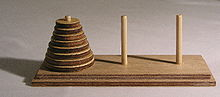
\includegraphics[width=0.57\textwidth]{figures/220px-Tower_of_Hanoi.jpeg}
\end{center}
\caption{Configurazione iniziale del puzzle classico della torre di Hanoi.}
\end{figure}

Ci sono tre pioli ('A','B' e 'C') su cui sono collocati $n$ dischi. Le configurazioni valide sono quelle in cui nessun disco si trova collocato sopra un disco più piccolo.
Nel puzzle classico (Édouard Lucas, 1883) viene richiesto di portarsi dalla configurazione in cui tutti i dischi risiedono sul piolo 'A' (detta \emph{configurazione iniziale}) alla \emph{configurazione finale} in cui tutti i dischi sono in 'C', spostando sempre un solo disco alla volta (mossa).
\'E nota l'elegante soluzione ricorsiva che risolve il puzzle classico col minimo numero di mosse. La soluzione ottima è di fatto unica anche se trova diverse descrizioni/rappresentazioni/interpretazioni in forma iterativa.

\begin{center}
  \animategraphics[loop,autoplay]{12}{./figures/animation/frame-}{0}{39}
\end{center}

Quì consideriamo la questione di rimettere a posto il puzzle nel minor numero possibile di mosse: partendo da una configurazione valida qualsiasi vogliamo riportarlo alla configurazione iniziale il più rapidamente possibile.
Per descrivere la generica configurazione valida è sufficiente specificare su quale piolo si trovi ciascuno degli $n$ dischi:
a quel punto la condizione di validità determina univocamente l'ordinamento dei dischi su ciascuno dei pioli. I dischi, dal più piccolo al più grande, sono numerati da $1$ ad $n$.

Per le istanze fino ad $n\leq 10$ dischi ti chiediamo di listare una per una le mosse (utilizza le funzioni rese disponibili nel template per non sporcarti le mani con la formattazione del tuo output). Per le istanze più grandi ti chiediamo di riportare solo le ultime $6$ cifre del numero di mosse, restituisci cioè il numero minimo di mosse $m$ modulo $1\,000\,000$ (ossia {\tt m\%1\,000\,000}). Infatti il valore di $m$ potrà divenire così grande da non poter essere memorizzato in una variabile del linguaggio scelto, non sono questioni che ci preme tu sappia affrontare in questo contesto.



\sezionetesto{Input ed Output}

Per la gestione pulita di input ed output consigliamo di utilizzare il template di soluzione fornito tra gli attachmets alla pagina del problema.
La prima riga del file \verb'input.txt' contiene il numero di dischi $n$,
la seconda riga contiene una stringa di lunghezza $n$ sull'alfabeto $\{A,B,C\}$,
il cui $i$-esimo carattere specifica il piolo su cui risiede il disco~$i$.
Nel caso in cui $n>10$, nel file \verb'output.txt' si scrive un unico numero naturale di massimo sei cifre decimali, ossia {\tt m\%1000000} dove $m$ è il minimo numero di mosse che è necessario spendere per riordinare il puzzle.
Altrimenti, nel caso in cui $n\leq 10$,  il file \verb'output.txt' si compone precisamente di $m$ righe, con la riga $i$-esima  che specifica la mossa $i$-esima come illustrato negli esempi. 


% Esempi
\sezionetesto{Esempio di input/output}

%In attachment alla pagina del problema trovate diverse copie input/output tra cui le seguenti.
%\vspace{0.5cm}

\esempio{
4

BACA
}{
Muovi il disco 1 dal piolo B al piolo C

Muovi il disco 2 dal piolo A al piolo B

Muovi il disco 1 dal piolo C al piolo B

Muovi il disco 3 dal piolo C al piolo A

Muovi il disco 1 dal piolo B al piolo C

Muovi il disco 2 dal piolo B al piolo A

Muovi il disco 1 dal piolo C al piolo A
}

\esempio{
11

CCAAAAAAAAA
}{3}

\esempio{
20

CCCCCCCCCCCCCCCCCCCC
}{48575}

% Assunzioni
\sezionetesto{Assunzioni e note}
\begin{itemize}[nolistsep, noitemsep]
  \item $0 \le n \le 30$.
\end{itemize}
  
\section*{Subtask}

  \begin{itemize}
    \item \textbf{Subtask 1 [0 punti]:} casi di esempio forniti alla pagina del problema, partendo dai tre casi sopra.
    \item \textbf{Subtask 2 [10 punti]:} $n \le 10$, torre assegnata in configurazione finale (tutti i dischi sul piolo 'C').
    \item \textbf{Subtask 3 [10 punti]:} $10 < n < 20$, torre assegnata in configurazione finale.
    \item \textbf{Subtask 4 [5 punti]:} $20 \le n < 22$, torre assegnata in configurazione finale.
    \item \textbf{Subtask 5 [5 punti]:} $n > 10$, torre assegnata in configurazione finale.
    \item \textbf{Subtask 6 [25 punti]:} $n \le 10$.
    \item \textbf{Subtask 7 [10 punti]:} $10 < n < 20$.
    \item \textbf{Subtask 8 [10 punti]:} $20 \le n < 22$.
    \item \textbf{Subtask 9 [25 punti]:} $n > 10$.
  \end{itemize}
  
